\documentclass[12p]{article}
\setlength{\parindent}{0em}
\usepackage{amsmath, mathrsfs, listings}
\usepackage{upquote, amssymb}
\usepackage[utf8]{inputenc}
\usepackage[english]{babel}
\usepackage[%
    left=0.50in,%
    right=0.50in,%
    top=1.0in,%
    bottom=1.0in%
]{geometry}%
\usepackage{graphicx}
\graphicspath{ {./images/} }
\renewcommand{\baselinestretch}{1.5}

\begin{document}

(1) Adjon formulát abszolút folytonos eloszlású X valószínűségi változó esetén az Y = g(X) valószínűségi változó várható értékére!

(2) Legyen X standard normális eloszlású valószínűségi változó. Számítsa ki az X várható értékét! 

(3) Mondja ki Bayes tételét. (3x)

Legyen B1, B2, ..., pozitív valószínűségű eseményekből álló teljes eseményrendszer, A $\in$ $\mathscr{A}$ pozitív valószínűségű. Ekkor

$$\displaystyle{P(B_k|A) = \frac{P(A|B_k)P(B_k)}{\displaystyle{\sum_i} P(A|B_i)P(B_i)}}$$

(4) Igazolja, hogy független azonos paraméterű binomiális eloszlású valószínűségi változók összege is ilyen.

(5) Írja fel az X és Y együttes eloszlásfüggvénye és az X perem eloszlásfüggvénye között fennálló kapcsolatot.

(6)  Definiálja a szórásnégyzetet és mondja ki legfontosabb tulajdonságait. (3x)

$$D^2X = E[(X - EX)]^2 = EX^2 - E^2X$$

Tulajdonságok:

\begin{itemize}
	\item $\sigma \geq 0$
	\item $\sigma = 0$ csak akkor teljesül, ha minden ismérvérték egyenlő.
	\item Ha minden ismérvértékhez hozzáadjuk ugyanazt a valós számot, a szórás változatlan marad.
	\item Ha minden ismérvértéket megszorozzuk ugyanazzal az a valós számmal, a szórás az a szám abszolútértékével szorzódik.
\end{itemize}

(7) Definiálja a konfidencia-intervallum fogalmát (3x)

A konfidenciaintervallum a valószínűségi intervallum, az induktív statisztika eszköze: ha mintából becsülünk, sosem tudjuk a pontos értéket, a teljes sokaság felmérése igen drága dolog. A konfidenciaintervallum adott szignifikanciaszinten: a becsült változó alsó és felső korlátja.

(8) Definiálja az első- és a másodfajú hiba fogalmát

(9) Adja meg a lineáris regresszió feladatát és megoldását

(10) Definiálja idősorok erős stacionaritását

(11) Definiálja az ASN fogalmát.

(12) írja fel az eloszás- és a sűrűségfüggvényeket karakterizáló tulajdonságokat! (3x)

Eloszlásfüggvény:\\
$F_X(z):=P(X<z)$. $F_X(z):\mathbb{R}\rightarrow\mathbb{R}$ függvény az X valószínűségi változó eloszlásfüggvénye.\\
Tulajdonságai:

\begin{itemize}
	\item $0 \leq F_X(z) \leq 1$
	\item $F_X(z)$ monoton nő
	\item $\lim_{z \rightarrow \infty} F_X(z) = 1; \lim_{z \rightarrow -\infty} F_X(z) = 0$
	\item $F_X(z)$ balról folytonos
\end{itemize}

Sűrűségfüggvény:\\
Az X valószínűségi változó sűrűségfüggvénye $f(x) \leftrightarrow X$-re:

$F_X(z) = \int_{-\infty}^z f(t) dt$

Tulajdonságai:
\begin{itemize}
	\item $f \geq 0$
	\item $\int_{-\infty}^{\infty} f(t) dt = 1$
	\item Minden ilyen f integrálfüggvénye eloszlásfüggvény
\end{itemize}

(13) Legyen X pascal eloszlású valószínűségi változó. Számítsa ki az X várható értékét!

(14) Mi a kapcsolat az X és Y valószínűségi változó függetlensége és együttes eloszlásfüggvénye között? (3x)

(15) írja fel, az X diszkrét valószínűségi változó várható értkének definícióját! (2x)

(16) -

(17) Vezesse le a polinomiális eloszlás koordinátái közötti korrelációra vonatkozó képletet.

(18) Definiálja a Poisson folyamatot. (3x)

Poisson folyamat: időben lejátszódó folyamatnál adott [a,b) intervallumba eső események száma $(X_{a,b})$ éppen $\lambda(b-a)$ paraméterő Poisson eloszlású, ha a folyamat

\begin{itemize}
	\item homogén: $X_{a,a+t}$ eloszlása csak t-tıl függ;
	\item utóhatás nélküli: $X_{a,b}$ és $X_{b,c}$ függetlenek ha a<b<c;
	\item nemelfajuló: $0<P (X_{a,b}=0)<1$.

\end{itemize}

(19) Mondja ki a nagy számok törvényének minél több változatát. (3x)

(20) Vezesse le a Poisson eloszlás paraméterére a maximum likelihood becslést. (3x)

Zyxon megoldasas:

A likelihood fuggveny:

$$L(\theta;\underline{x}) = f_{\theta}(\underline{x}) = \prod^n_{i=1} f_{\theta}(x_i)$$

Ennek maximumhelye lesz a $\theta$ paraméter maximum likelihood becslése. A Poisson-eloszlás paramétere: $\overline{X}$

Tankonyvar.hu-s megoldas:

$$P(X_1 = k) = \frac{\lambda^k}{k!}e^{-\lambda}\quad k=0, 1, 2, ...$$
A likelihood-fuggveny
$$L(x_1, ..., x_n;\lambda)=\prod^n_{i=1}\frac{\lambda^{x_i}}{x_i!}e^{-\lambda}$$
A loglikelihood-fuggveny
$$l(x_1, ..., x_n;\lambda) = \sum^n_{i=1}(x_i log \lambda - \lambda - log x_i!)$$
A maximumhelyet derivalassal hatarozzuk meg:
$$0 = \frac{\theta l(x_1, ..., x_n;\lambda)}{\theta \lambda} = \frac{1}{\lambda} \sum^n_{i=1} x_i - n$$
Innen
$$\hat{\lambda} = \frac{1}{n} \sum^n_{i=1} X_i = \overline{X}$$
A maximum-likelihood becsles.

(21) Definiálja a lineáris modell hipotéziseit és adja meg a próbastatisztikát.

(22) Legyen X +1 és -1 értéket felvevő valószínűségi változó, $P(X = 1) = 1/6$ és $P(X = -1) = 5/6$. Számítsuk ki X várható értékét és szórás négyzetét.

(23) Bizonyítsa be a nagy számok gyenge törvényét. (2x)

(24) Legyen $X^2$ egyenletes a $[0, 1]$-en. Adja meg X eloszlását és várható értékét.

(25) Irja fel a rendezett minta k-adik elemének a sűrűségfüggvényét.

(26) Rajzolja fel, hogyan lehet a sűrűségfüggvények segítségével a próbák kritikus értékeit és erőfüggvényüket szemléltetni!

(27) Definiálja a $\chi$-négyzet próbát és adja meg legfontosabb alkalmazásait.

(28) Adja meg a lineáris regresszió feladatát és alkalmazásait.

(29) Vezesse le a normális eloszlás várható értékére a momentum módszerrel adódó becslést.

(30) Adjon módszert idősorok simítására.

(31) Definiálja a szórásnégyzetet és mondja ki legfontosabb tulajdonságait.

(32) Mondja ki a centrális határeloszlás tételt. (2x)

151.-es kerdesben benne van a valasz.

(33) Legyen $X$ olyan valószínűségi változó, amely a (0, 1) intervallumból veszi fel az értékeit. Eloszlásfüggvénye ott F(t) = t/2 ha $t \in (0, 1/2]$, és $F(t) = 3/4 + t/4$ ha $t \in (1/2, 1]$. Rajzoljuk fel X eloszlásfüggvényét és számítsuk ki a $P(X \leq 1/2)$, valamint a $P(1/4 \leq X \leq 3/4)$ és $P(X = 1/2)$ valószínűségeket!

(34) Definiálja a teljes eseményrendszer fogalmát! (2x)

Események $A_1, A_2, ...,$ sorozata teljes eseményrendszer, ha
egymást páronként kizárják és egyesítésük $\Omega$.

(35) Definiálja a folytonos eloszlásokra a várható érték fogalmát.

(36) Mondja ki Bernstein tételét.

Legyen $(X_1, X_2, ..., X_n)$ olyan, hogy $D^2(X_1) + D^2(X_2) ... + D^2(X_n) < kn$, valamint tegyük fel, hogy van olyan $h: N \rightarrow R_{+}$ függvény, melyre $|R(X_i, X_j)| \leq h(|i-j|)$ és $\frac{1}{n} \displaystyle{\sum^n_{i=1}} h(i) \rightarrow 0$ ekkor $(X_1 + ... + X_n) / n - (m_1 + m_2 + ... + m_n)/n \rightarrow 0$ sztohasztikusan.

(37) Bizonyítsa be a Markov egyenlőtlenség általános alakját.

77.-es kerdesben!

(38) Definiálja a maximum-likelihood módszert.

Azt a paraméterértéket keressük, ahol a likelihood függvény a legnagyobb értéket veszi fel (azaz diszkrét esetben az
ismeretlen paraméter azon értéket keressük, amely mellett a bekövetkezett eredmény maximális valószínűségű): $\max_{\theta}L(\theta; x)$.

Ez nyilván megegyezik azzal a paraméterértékkel, ahol a log-likelihood függvény veszi fel a legnagyobb
értéket, azaz: $\max_{\theta} l(\theta; x)$.

Amennyiben a függvény deriválható $\theta$ szerint, akkor a maximumot kereshetjük a szokásos módon, a deriváltak
segítségével, azonban a feladatunkat jelentősen megnehezíti, hogy olyan n-szeres szorzatot kellene deriválni, amelyiknek minden tagjában ott van az a változó, ami szerint deriválnunk kellene. Ezért likelihood függvény helyett a log-likelihood függvény maximumhelyét keressük.

Ha $\theta$ 1 dimenziós, akkor $\partial_\theta l(\theta, x) = 0$, míg ha $\theta = (\theta_1, ..., \theta_p)$ p dimenziós, akkor $\partial_{\theta_i} l(\theta, x) = 0$ megoldásából
kapjuk a becslést. (A második deriváltak segítségével ellen ˝orizz¨uk, hogy valóban maximum.)


(39) Definiálja a Wilcoxon próbált.

Ez a próba olyan kísérleti helyzetekben alkalmazható, ahol a mintavétel a páros megfigyelésen alapul, ahol 2 összefüggő változóból mintavétel történik, úgy, hogy mindegyikből egy-egy jut egy megfigyelési egységbe.

A próba feltételei:
\begin{itemize}
	\item Ordinális skálán mérhető folytonos valószínűségi változók esetén akkor alkalmazható,
	\item ha a különbségek is ordinális skálán mérhetőek.
	\item Erősen asszimmetrikus eloszlás esetén nem alkalmazható.
\end{itemize}

(40) Definiálja az autoregressziós és a mozgóátlag folyamatokat.

$$??$$

(41) Mit jelent a becsléses illeszkedésvizsgálat és hogyan alkalmazzuk rá a $\chi$-négyzet próbát?

(42) Legyen X n-edrendű p paraméterű binomiális eloszlású valószínűségi változó. Számítsa ki az X várható értékét! 

(43) Mondja ki a szita (Poincaré) formulát.

Képlet az általános esetre:

$$P(A_1 \cup A_2 \cup ... \cup A_n) = \sum^n_{i=1} (-1)^{i+1} S^{(n)}_i$$
ahol
$$S^{(n)}_i = \sum_{1 \leq j_1 < j_2 < ... < j_i \leq n} P(A_{j_1}, \cap A_{j_2} \cap ... \cap A_{j_i})$$

az i tényezıs metszetek
valószínőségeinek összege.

(44) Definiálja a kovarianciát és írja le tulajdonságait. (4x)

$cov(X,Y) := E[(X-E(X))(Y-E(Y))]$

Kiszámítása:
$cov(X,Y) = E(XY)-E(X)E(Y)$

Ha X és Y függetlenek $\rightarrow$ $cov(X,Y) = 0$, fordítva nem feltétlenül igaz

A kovariancia szimmetrikus: $cov(X,Y) = cov(Y,X)$

$cov(X,X) = D^2(X)$

(45) Mondja ki a centrális határeloszlás tétel lokális változatát. (2x)

Legyenek $X_1 , X_2 ,..., X_n ,...$ független, azonos eloszlású, abszolút folytonos valószínőségi változók. Tegyük fel, hogy $\sigma_2=D_2(X)$ véges $(m:=E(Xi))$ és hogy $f(x)$ korlátos. Tekintsük a standardizált összegüket:

$$Z_n := \frac{X_1 + ... + X_n - nm}{\sqrt{n}\sigma}$$

Ekkor $Z_n$ sűrűségfüggvénye konvergál a standard normális
eloszlás sőrőségfüggvényéhez, azaz

$$\lim_{n \rightarrow \infty} f_n(x) = \frac{1}{\sqrt{2\pi}} e^{- \frac{x^2}{2}}$$

A konvergencia z-ben egyenletes.

(46) Legyen X egyenletes a [0,1]-en. Adja meg $X^2$ eloszlását és várható értékét.

(47) Irja fel a Nadarajah módszer lényegét és szemléltesse grafikusan az eljárás motivációját! 

Ha csak mért adataink vannak, közelítjük a
feltételes várható értéket (hasonló a ParzenRosenblatt becsléshez).

$$\hat{r}_n(x) = \frac{\displaystyle{\sum^n_{i=1} Y_ik \left(\frac{x - X_i}{h_n}\right)}}{\displaystyle{\sum^n_{i=1} k \left(\frac{x - X_i}{h_n}\right)}}$$

A Parzen-Rosenblatt tétel feltételei esetén ez
konzisztens becslése az E(Y|X) regressziónak.

(48) Definiálja a 2 mintás t-próbát és vezesse le a próbastatisztika képletét! 

(49) Mondja ki a Neyman-Pearson lemmát!

(50) Definiálja az autokorrelációs együtthatókat és adja meg becslésüket arra az esetre, amikor reziduálisokból számolunk! 

(51) Definiálja a valószínűségi mező fogalmát! (2x)



(52) Vezesse le, hogy a korrigált tapasztalati szórásnégyzet torzítatlan becslés a szórásnégyzetre. 

(53) Vezesse le, hogy a relatív gyakoriság konzisztens becslés a valószínűségre.

(54) Definiálja becslések aszimptotikus torzítatlanságát.

(55) Definiálja a t-próbát az egy- és kétmintás esetre is.

(56) Definiálja a szekvenciális próbát (egyszerű hipotézisek esetére).

(57) Definiálja a korrelációs együtthatót és mondja ki legfontosabb tulajdonságait.

(58) Mikor nevezünk egy torzítatlan becslést hatásosabbnak egy másiknál?

(59) Definiálja idősorokra a trend és a periódus fogalmát.

(60) Adjon példát olyan maximum likelihood becslésre, ami nem torzítatlan! (3x)

(61) Mondja ki abszolút folytonos valószínűségi változók függetlenségének ekvivalens jellemzőit.

(62) Definiálja valószínűségi változók eloszlását.

Mivel a gyakorlati problémáknál $\Omega$ nem
mindig adható meg egyértelműen, és
absztrakt halmazok helyett szívesebben
dolgozunk a valós számokkal, a kulcsfogalom
a valószínűségi változók eloszlása.\\
Legyen B tetszőleges Borel halmaz.
$Q_X(B):= P{\omega: X(\omega) \in B}$ valószínűséget ad
meg R Borel halmazain. Ez az X eloszlása.\\

(63) Mit jelent a valószínűség folytonossága?

(64) Definiálja n valószínűségi változó függetlenségét.

 Az $X_1,...,X_n$ valószínűségi változók függetlenek, ha az $\mathscr{F}_{X1}, \mathscr{F}_{X2} ,...,\mathscr{F}_{X_n}$ generált $\sigma$-algebrák függetlenek.

(65) Definiálja diszkrét valószínűségi változók együttes eloszlását!

az X diszkrét valószínűségi változó, ha értékkészlete $(x_1 ,..., x_n...)$ legfeljebb megszámlálható.\\
A valószínűségi változó definíciójából adódóan $\{\omega:X(\omega)= x_i\}=\{X=x_i\}= \in \mathscr{A}$ azaz $p_i:=P$ $(X=x_i)$értelmes. Ezek meg is határozzák X eloszlását.

(66) Definiálja a t eloszlást!

(67) Definiálja a gyenge konvergenciát!

(68) Irja fel annak a valószínűségét, hogy a 90/5-ös lottónál egy szelvénnyel játszva legalább 2 találatunk lesz!

(69) Legyen az alábbi 3 megfigyelésünk az $(X, Y)$ párra. $(1;2)$ $(1.2;2.5)$ $(0.8;1.6)$. Nadarajah
módszerét használva a $k(x) = 1$, ha $-1/2 < x < 1/2$ (és 0 különben) magfüggvénnyel és a $h = 0.5$ ablakszélességel, mi lesz az $E(Y|X = 1.1)$ becslése?

(70) Vezesse le egyszerű hipotézisekre, hogy az egymintás u-próba valószínűséghányadospróba az egyoldali ellenhipotézis esetén!

(71) Hogyan tudjuk a lineáris modellt alkalmazni polinommal történő közelítésre?

(72) Adjon példát olyan maximum likelihood becslésre, mely nem torzítatlan.

(73) Definiálja az előjelpróbát! Mik a kritikus értékek? (3x)

Nemparaméteres próba, illeszkedésvizsgálat $\rightarrow$ adott eloszlású-e a minta?

Az előjelpróba a különbségek előjelén alapul. $H_0$ esetén Binom(n; 1/2).

(74) Adjon példát olyan $X_n$ valószínűségi változó-sorozatra, amely független tagú, de mégsem teljesül rá a centrális határeloszlástétel.

(75) Legyen X egyenletes eloszlású a [-1, 1] intervallumon. Számítsa ki $X^2$ sűrűségfüggvényét.

(76) Definiálja a normális eloszlást és vezesse le a legfontosabb tulajdonságait.

(77) Mondja ki és bizonyítsa is be a Markov egyenlotlegnséget.

Legyen $g : \mathbb{R} \rightarrow \mathbb{R}$ monoton növő pozitív függvény, $X \geq 0$ valószínűségi változó, melyre $EX < \infty$ és $\mathcal{E} > 0$ tetszőleges. Ekkor

$$P(X \geq \mathcal{E}) \leq \frac{E(g(X))}{g(\mathcal{E})}$$

Spec., ha $g(x) = x$, akkor

$$P(X \geq \mathcal{E}) \leq \frac{EX}{\mathcal{E}}$$

Bizonyitas diszkret esetre

$$E(X) = \sum_{i \in R_X} i*p_i = \sum_{i>0,i\in R_X} i*p_i \geq \sum_{i \geq a, i\in R_X} i*p_i \geq \sum_{i\geq a, i\in R_X} a*p_i = aP(X \geq a)$$

Bizonyitas folytonos esetre

$$E(X) = \int_{-\infty}^{\infty} yf_X(y)dy = \int_{0}^{\infty} yf_X(y)dy \geq \int_{a}^{\infty} yf_X(y)dy$$
$$\int_{a}^{\infty}yf_X(y)dy \geq \int_{a}^{\infty} af_X(y)dy = a * P(X \geq a)$$

(78) Hogyan alkalmazhatjuk a Kolmogorov-Szmirnov próbát véletlenszám-generátorok tesztelésére?

A tapasztalati és az elméleti eloszlásfüggvény
legnagyobb eltéréseit karakterizálja

$$K_n^{+} = \sqrt{n} \max (F_n(x) - F(x)), \quad K_n^{-}=\sqrt{n} \max(F(x) - F_n(x))$$

Táblázatból kiolvasható a keresett valószínűség\\
A kis lokális eltéréseket nem mutatja ki

(79) Definiálja a binomiális eloszlást, vezesse le a képletét és adja meg alkalmazási lehetőségeit!

(80) Legyenek az adataink: 1,2,5,6. Számolja ki a mediánt és rajzolja fel a tapasztalati eloszlásfüggvényt!

(81) Tegyük fel, hogy egy 1ö fős csoportban mindenki kihúzza valakinek a nevét a karácsonyi ajándékozásnál. várható értékben hány ember húzta saját magát? Vezesse is le az eredményt!

(82) Rajzolja fel a $\lambda = 1$ és $\lambda = 2$ paraméterű exponenciális eloszlás sűrűség- és eloszlásfüggvényét!

(83) Vezesse le a $[0, \theta]$ intervallumon egyenletes eloszlásra a maximum likelihood becslést n mintaelem alapján!

(84) Rajzolja fel az alábbi minta tapasztalati eloszlásfüggvényét: 1,5,6,7! (2x)

(85) Hogyan tudunk inverz módszerrel véletlen számot generálni? (2x)

Legyen X val. vált., F eloszlásfüggvénnyel,
amely monoton növekedı és folytonos. Ekkor

\begin{itemize}
	\item F(X) egyenetes eloszlású [0, 1]-en.
	\item Ha $U \sim U(0, 1)$ akkor $F^{-1}(U)$ eloszlásfüggvénye F.
\end{itemize}

Pl.:

$$X \sim exp(\lambda) \rightarrow F(x) = 1-exp(-\lambda x) \rightarrow F^{-1}(x) = -\ln (1-x)/\lambda \rightarrow -\ln(1-U)/\lambda \sim exp(\lambda)$$

(86) Legyen az X valószínűségi változó sűrűségfüggvénye $f(x) = x^2/9$, ha $0 < x < 3$ és $0$ különben. Adjuk meg $X$ eloszlásfüggvényének értékét az $1/2$ helyen. $E(1/X)=?$ Adjuk meg $sqrt{X}$ sűrűségfüggvényének értékét az $1/2$ helyen.

(87) Számítsa ki annak a valószínűségét, hogy egy háromgyerekes családban azonos neműek a gyerekek! (Tegyük fel, hogy a fiúk és lányok szóletési valószínűsége is 0.5 és hogy az egyes születések függetlenek.)

(88) Definiálja a várható érték fogalmát diszkrét valószínűségi változókra!

A $p_i =P (X=x_i)$ eloszlással megadott valószínőségi változó várható értéke $E(X):= p_1x_1+ p_2x_2 +...,$ ha a sor abszolút konvergens.

(89)  Legyen X egyenletes eloszlású a $[-2,2]$ intervallumon. Adja meg $(X - 2)(X + 2)$ sűrűségfüggvényét.

(90) Mondja ki abszolút folytonos valószínűségi változók függetlenségének ekvivalens jellemzőit.

Ha X koordinátái függetlenek, akkor definíció szerint:

$F_X(z) = P(X_1<z_1, X_2<z_2, ..., X_d<z_d) = F_1(z_1)F_2(z_2)...F_n(z_n) \forall z \in \mathbb{R}^d$

(91) Mondjon példát az egyenletes, az exponenciális és a normális eloszlás alkalmazására!

Egyenletes eloszlás:\\
Véletlengenerátorokban igyekeznek az egyenletes eloszlást egy adott intervallumon minél inkább közelíteni

Exponenciális eloszlás:\\
Előrejelzéseknél alkalmazzák: n adatpontos minta megfigyelése után egy ismeretlen exponenciális eloszlású forrásból meg tudjuk jósolni, hogy mi lesz a következő érték ugyanabból az ismeretlen exponenciális eloszlású adatforrásból

Normális eloszlás:\\
Mérési hibákra, mért ingadozásokra és olyan élettartam vizsgálatokra használjuk, ahol a készülékek, alkatrészek rendszeres kopással mennek tönkre. Bizonyos feltételek eseték a binomiális eloszlás közelítésére is használható.

(92) Definiálja a bootstrap módszert.

\begin{itemize}
	\item Adott $X_n$-ből m elemű visszatevéses mintát veszünk (általában m=n) \quad $X^{*}_m = \{X^{*}_1,...,X^{*}_m\}$
	\item $X_i^{*}$ közös eloszlása: $F_n = n^{-1} \sum^n_{i=1} \delta_{x_i}$
	\item $T^{*}_{m,n} = t_m (X^{*}_m;F_n)$
	\item Ismétlés $\rightarrow \hat{G}_{m,n}$
	
\end{itemize}


(93) Mi a leíró statisztika feladata?

Célja egy már rendelkezésre álló, valóságra vonatkozó adathalmaz összefoglalása, elemzése, egyszóval az információtömörítés.\\

(94) Definiálja a kovarianciát!

$$cov(X, Y) = E(XY) - EXEY$$

(95) Mihez tart $P(X1+X2+ ... +Xn > 9n/2)$, ha $X1, X2, . . .$ független, a $[4,6]$ intervallumon
egyenletes eloszlású valószínűségi változók és n tart végtelenhez?

(96) Vezesse le az exponenciális eloszlás várható értékére vonatkozó képletet!

(97) Legyen az alábbi 3 megfigyelésünk az $(X, Y)$ párra. $(1;2)$ $(1.3;2.5)$ $(0.8;1.5)$. Nadarajah
módszerét használva a a $k(x) = 1$, ha $-1/2 < x < 1/2$ (és 0 különben) magfüggvénnyel és a $h = 0.5$ ablakszélességgel, adjon becslést $Y$ közelítésére, ha $X = 1$.

(98) Definiálja az egy-és kétmintás u-próbát.

Egymintás:\\
$H_0: m=m_0; H_1 m \neq m_0$. Ha ismert a szórás:
$$u = \sqrt{n}\frac{\overline{x} - m_0}{\sigma}$$

Ketmintas:
\begin{itemize}
	\item Első minta: n elemű, $\sigma_1$ szórású
	\item Második minta: m elemű, $\sigma_2$ szórású
\end{itemize}

Ha ismert $\sigma$:

$$u = \frac{\overline{X} - \overline{Y}}{\sqrt{\frac{\sigma^2_1}{n} + \frac{\sigma^2_2}{m}}}$$

(99) Az alábbi minta: 0,0,1,1,2 alapján becsüljük torzítatlanul az alábbi paramétereket:
várható érték, szórásnégyzet, annak a valószínűsége, hogy $X > 0.2$.

(100) Adjon módszert arra, hogyan szimulálna véletlen számot a $\sin x (0 < x < \pi/2)$ sűrűségfüggvényű eloszlásból!

(101) Hogy hívjuk a $h(t) = E(|X - t|^2)$ függvény minimum helyét?

(102) Hogyan adhatjuk meg a megszámlálható valószínűségi mezőn a valószínűséget?

(103) Legyen X 5 várható értékű és 2 szórású normális eloszlású, Y pedig az X = 7 esemény indikátora. Számítsa ki Y várható értékét és szórását!

(104)  Definiálja a visszatevés nélküli mintavétel modelljét és adja meg a különböző selejtszámok valószínűségeit!

(105) Mondja ki a Markov egyenlőtlenséget!

77.-es kerdesben!

(106) Vezesse le a valószínűségre a maximum likelihood becslést n mintaelem alapján!

(107) Definiálja a sztochasztikus konvergenciát! (2x)

 minden $\mathcal{E}$, $\delta>0$-
hoz megadható olyan $n_0$, hogy $n>n_0$ esetén $P(|X_n-X| \geq \mathcal{E}) \leq \delta$.

Lemma

$$X_n \rightarrow X m.m. \leftrightarrow \lim_{m \rightarrow \infty} P(\sup_{n \geq m} |X_n - X| > \mathcal{E}) = 0$$

Köv.: A m.m. konvergenciából következik a
sztochasztikus konvergencia.


(108) Írja le a sűrűségfüggvény becslésére tanult eljárást.

$$f_n(x) = \frac{1}{nh_n}\sum^n_{i=1}k\left( \frac{x-X_i}{h_n} \right)$$

(109) Adja meg a legkisebb négyzetes becslést a lineáris modellben. Mik a tulajdonságai?

(110) Legyen X egyenletes a $[0, 1]$-en. Adja meg $X^2$ eloszlását és várható értékét.

(111) Számolja ki a Wilcoxon próbastatisztika értékét az alábbi két adatsorra! Hogyan döntene arról, hogy tekinthetők-e azonos eloszlásból származónak? Az első minta: 1,2,4,12,23,50;
a második minta: 3,8,15,25,61,200.

(112) Definiálja az F-próbát és adja meg legfontosabb alkalmazásait. (2x)

$$H_0: \sigma_1 = \sigma_2$$
$$H_1: \sigma_1 \neq \sigma_2$$
Probastatisztika
$$F= \frac{(s_1^{*})^2}{(s_2^{*})^2} \stackrel{H_0 eseten}{\sim} F_{n-1,m-1}$$

(113)  Hogyan generálhatunk véletlen számot Neumann módszerével?

Legyen f(x) tetszőleges sűrűségfüggvény, $g(x)$ pedig olyan sűrűségfüggvény, amelyre $f(x) < Mg(x)$, valamely $M>1$ esetén és $g(x)$-ből könnyen tudunk mintát venni (tipikus példa az egyenletes eloszlás).

(114) Töltse ki az alábbi táblázat hiányzó celláit úgy, hogy a peremeloszlások egyenletesek
legyenek a megadott számokon! Függetlenek-e ezek a változók? Számolja ki az $E(X^2Y)$ várható értéket!

\begin{center}
 \begin{tabular}{| c c || c | c | c | c |} 
 \hline
 Y & X &  0 & 1 & 2 & 3\\ [0.5ex] 
 \hline\hline
 0 &  & 0,2 & & 0,05 & \\ 
 \hline
 1 &  & & 0,15 & & \\
 \hline\hline
\end{tabular}
\end{center}

(115) Mutassa meg, hogy független azonos paraméterű binomiálisok összege binomiális eloszlású! Mi a kapcsolat a rendek között?

(116) Definiálja két esemény függetlenségét!

Az A és B események függetlenek, ha $P(A \cap B) = P(A)P(B)$.

(117) Számítsa ki két kockadobás maximumának a várható értékét.

(118) Definiálja az első- és másodfajú hiba fogalmát, valamint próbák konzisztenciáját.

Első:\\
Valamely nullhipotézis statisztikai próbával végzett vizsgálatában az a hiba, amelyet a nullhipotézis elutasítása jelent amikor az igaz. Valószínûsége az elsõfajú kockázat (alfa). 

Másodfajú hiba\\
Az a hibás döntés, hogy nem vetjük el a helytelen nullhipotézist abban az esetben, amikor az alternatív hipotézis igaz. A próba közvetlenül nem ellenõrzi, ezért ha a próba nem utasítja el a nullhipotézist, ez még nem jelenti azt, hogy a nullhipotézist megfelelõ statisztikai biztonsággal elfogadhatjuk. Valószínûsége a másodfajú kockázat (béta). 



(119) Irja le a t-próba alkalmazását a párosított megfigyelések esetére.

(120) Vajon van-e stacionárius megoldása az $X_n = 0.96 X_{n-1} + \epsilon_n$ rekurziónak? Válaszát
indokolja!

(121) Legyen a mintaelemek sűrűségfüggvénye $f(x) = (\theta + 1)x^{\theta}$ ha $0 < x < 1$ ($\theta \geq$ 0 a par.).
Egy mintaelem alapján határozzuk meg az $\alpha = 0.05$ terjedelmű valószínűséghányadospróbát a $H_0 : \theta = 0, H_1 : \theta = 1$ hipotézisekre!

(122) Ismertesse a lineáris regresszió együtthatóira vonatkozó próbák lényegét! (2x)

??

(123) Adott n elemű minta az alábbi eloszlásból: $P(Z = 1) = c$, $P(Z = 2) = 2c$, $P(Z = 3) = 1 - 3c$ ($0 < c < 1/3$ az ismeretlen paraméter). Határozza meg a paraméter maximum likelihood becslését!

(124) Számítsa ki két kockadobás minimumának a várható értékét.

(125) Írja fel a Csebisev egyenlőtlenséget, és vázolja a bizonyítását.

Legyen X tetszőleges valószínűségi változó, melyre $D^2X < \infty$ és $\mathcal{E} > 0$ tetszőleges. Ekkor

$$P(|X - EX| \geq \mathcal{E}) \leq \frac{D^X}{\mathcal{E}^2}$$

Bizonyítás:

???

(126) Legyen X 5 várható értékű Poisson eloszlású, Y pedig az X = 5 esemény indikátora. Számítsa ki Y várható értékét és szórását!

(127) Adjon példát olyan maximum likelihood becslésre, mely nem torzítatlan.

pl. a normális eloszlás szórásnégyzetére kapott becslés ilyen

(128) Adja meg a Wilcoxon-próba hipotéziseit, a próbastatisztikát és a kritikus tartományt.
Mikor alkalmazná ezt a próbát? (2x)

???

(129) Adjon meg két módszert integrálok szimulációval történő kiszámítására! Hasonlítsa is
össze őket!

\begin{itemize}
\item Integrálok közelítése
\item Bootstrap
\end{itemize}

Az első eljárás is torzítatlan és szórásnégyzete $(E(g^2(X)) - I^2) / N$, amiből kisebb szórás adódik.\\
Tovább is javítható, ha X az [a,b]-ra koncentrálódó f sűrűségfüggvényű eloszlásból származik:
$$\int^b_a g(x)dx = \int^a_b \frac{g(x)}{f(x)} f(x)dx = E (\frac{g(X)}{f(X)})$$
és ennek még kisebb a szórása, ha $f(X) \approx g(X)$\\
Tehát g(X)/f(X) szimulált értékeinek átlaga jó közelítés\\
Az is előnye, hogy improprius integrálokra is alkalmazható (ha pl. f a normális eloszlás)


(130) Definiálja a 2 mintás t-próbát és vezesse le a próbastatisztika képletét!

$$t = \sqrt{\frac{nm}{n+m}}\frac{\overline{X} - \overline{Y}}{\sqrt{\frac{(n-1)(s^*_1)^2 + (m-1)(s^*_2)^2}{n+m-2}}} \stackrel{H_0 eseten}{\sim}
t_{n+m-2}$$

(131) -

(132) Vezesse le a normális eloszlás várható értékére a maximum likelihood becslést n mintaelem alapján!

$$L(\mu, \sigma^2;x) 
= \prod^n_{k=1} \frac{1}{\sqrt{2\pi \sigma^2}} 
e^{\frac{(x_i-\mu)^2}{2\sigma^2}}
=\left(\frac{1}{\sqrt{2\pi \sigma^2}}\right)^n 
e^{-\frac{1}{2 \sigma^2}} \sum^n_{k=1} (x_i - \mu )^2$$

$$\ln L(\mu, \sigma^2;x) = - \frac{n}{2} \ln 2\pi - \frac{n}{2} \ln \sigma^2 - \frac{1}{2\sigma^2} \sum^n_{k=1} (x_i - \mu)^2$$
$$(\ln L(\mu,\sigma^2;x))^{'}_{\mu} = - \frac{1}{2\sigma^2}(-2)\sum^n_{k=1}(x_i - \mu)$$

Átrendezve $(\ln L(\mu,\sigma^2;x))^{'}_{\mu} = 0$ egyenletet, kapjuk, hogy $\displaystyle{\hat{\mu} = \frac{\sum^n_{k=1} X_i}{n} = \overline{X}}$. Ez valóban maximum, mivel $(\ln L(\mu,\sigma^2;x))^{''}_{\mu} = -\frac{n}{\sigma^2} < 0$

(133) Írja fel, az X diszkrét valószínűségi változó várható értékének definícióját és sorolja fel
a várható érték legfontosabb tulajdonságait!

Egy X valószínűségi változó várható értéke

\begin{itemize}
	\item diszkrét esetben
		$$E(X) := \sum_k x_k P(X = x_k) = \sum_k x_k p_k$$
		
	\item folytonos esetben
		$$E(X) := \int_{-\infty}^\infty xp(x)dx$$
\end{itemize}

Nem minden valószínűségi változónak van véges várható értéke\\
Ha $E(X)$ véges, akkor az abszolút konvergencia miatt egyértelmű is.\\
Ha $EX$ véges, akkor $E(aX+b)=aEX+b$\\
Ha $EX$ és $EY$ véges, akkor $E(X+Y)=EX+EY$

(134) Legyen $\Omega = {1, 2, 3, 4, 5, 6}$, $P(i) = 1/6 (1 \leq i \leq 6)$ és $A = {1, 2, 3}$. Adon meg olyan B
eseményt, amire $0 < P(B) < 1$ és B és A függetlenek! Válaszát indokolja.

 Például $B = \{3, 4\}$, mert ekkor $P(A \cap B) = 1/6$ és $P(A)P(B) = \frac{1}{2} * \frac{1}{3}$, tehát egyenlőek, azaz a két esemény független.

(135) Tegyük fel, hogy az X valószínűségi változó sűrűségfüggvénye $f(x) = 2(1-x)$ ha $0 < x < 1$ és 0 különben. E(X) =? 

$$EX = \int^1_0 xf(x)dx = ... = 1/3$$

(136) Legyen az X valószínűségi változó eloszlása $P(X = k) = (5 - k)/15$, $ha 0 \leq k \leq 4$. $D^2(X)$ = ?

$D^2(X) = E(X^2) - E^2(X)$,$E(X) = 1 * \frac{4}{15} + 2 * \frac{3}{15} + 3 * \frac{2}{15} + 4 * \frac{1}{15} = \frac{20}{15}$.\\
$E(X^2) = 1 * \frac{4}{15} + 4 * \frac{3}{15} + 9 * \frac{2}{15} + 16 * \frac{1}{15}$.

(137) Mondja ki a nagy számok Bernoulli-féle törvényét!

A nagy számok törvényének legelső verzióját
még Bernoulli bizonyította,
indikátorváltozókra: eszerint azonos
körülmények között elvégzett független
kísérleteknél tetszőleges esemény relatív
gyakorisága tart az esemény
valószínűségéhez.

(138) Definiálja egy valószínűségi változó mediánját.

Az x valószínűségi változó mediánját $\overline{x}$ vagy $\mu_{1/2}(x)$ jelöli.
Páratlan elemszám esetén a középső elem, páros elemszám esetén a két középső elem átalaga.

(139) Mi a lényeges különbség a leíró és a matematikai statisztika között?

Leíró:\\
Célja egy már rendelkezésre álló, valóságra vonatkozó adathalmaz összefoglalása, elemzése, egyszóval az információtömörítés.\\
Matematikai:\\
Célja a megfelelő – vagyis a sokaság egészének paramétereit legjobban tükröző, reprezentáló – minta kiválasztása, a sokasági paramétereknek a minta paramétereivel történő becslése, illetve a sokasági paraméterekre vonatkozó feltételezések, hipotézisek elfogadása vagy elvetése. Foglalkozik továbbá a valóság összefüggéseinek egyszerűsített megragadására törekvő modellekkel is, mint az idősor- és regressziós modellek.

(140) Vezesse le a maximum likelihood becslést a binomiális eloszlás p paraméterére (az n paramétert tekintsük ismertnek)!

$$L(m, p; x) = \prod_{k=1}^n \displaystyle{\left({m \atop x_k}\right)}p^{x_k}(1-p)^{m-x_k} \quad (x_k = 0, 1, ..., m)$$
$$\ln L(m, p; x) = \sum^n_{k=1} \ln \left ({m \atop x_k}\right) + \ln p \sum^n_{k=1} x_k + \ln(1-p) \sum^n_{k=1}(m-x_k)$$
$$(\ln L(m,p;x))^{'}_p = \frac{1}{p} \sum^n_{k=1}x_k + \frac{1}{1-p} \sum^n_{k=1} (m - x_k) = \frac{1}{p} \sum^n_{k=1}x_k + \frac{1}{1-p}
\left(nm- \sum^n_{k=1}x_k \right) = \frac{1}{p}n\overline{x} + \frac{1}{1-p}(nm-n\overline{x})$$

Átrendezve a $(\ln L(m,p;x))^{'}_p = 0$ egyenletet, kapjuk, hogy $\hat{p} = \frac{\overline{X}}{m}$.  Ez valóban maximum, mivel $(\ln L(m,p;x))^{''}_p$-t kiértékelve a $\hat{p}$ helyen $(\ln L(m,p;x))^{''}_p = \frac{-n \overline{x}}{p^2} + \frac{-n(m-\overline{x})}{(1-p)^2}=
-n\left(\frac{\overline{x}}{p^2}+\frac{m - \overline{x}}{(1-p)^2}\right)<0$.

(141) Definiálja a hipotézisvizsgálat alapfogalmait!

Hipotézis: állítás, aminek igazságát vizsgálni szeretnénk
Statisztikai próba: eljárás, aminek a segítségével döntést hozhatunk a hipotézisről
Nullhipotézis: $H_0 : \theta \in \Theta$\\
Ellenhipotézis: $H_1 : \theta \in \Theta$\\
Paramétertér: $\Theta = \Theta_0 \cup \Theta_1$\\
Mintater: $\chi = \chi_e \cup \chi_k$\\
$\chi_k$: kritikus tartomány - azon X megfigyelések halmaza, amikre elutasítjuk a nullhipotézist\\
$\chi_e$: elfogadási tartomány - azon X megfigyelések halmaza, amikre elfogadjuk a nullhipotézist\\
A $\chi$ mintatér felosztását egy $T : X \rightarrow R$ statisztika (neve: próbastatisztika) segítségével végezzük el\\
P(elsőfajú hiba) = $\alpha(\theta) = P_\theta$ (elvetjük $H_0$-t $|$ $H_0$ igaz)\\
Terjedelem: $\alpha = sup\{\alpha(\theta) : \theta \in \Theta_0\}$\\
P(másodfajú hiba) = $\beta(\theta) = P_\theta$ (elfogadjuk $H_0$-t $|$ $H_0$ hamis)\\
Erőfüggvény: $\Psi(\theta) = 1 - \beta(\theta) = P_\theta$ (elvetjük $H_0$-t $|$ $H_0$ hamis)

(142)  Definiálja az u-próbát az egy- és kétmintás esetre is.

Egymintas

$$T(X) = u = \frac{\overline{X} - m_0}{\frac{\sigma}{\sqrt{n}}} \stackrel{H_0 eseten}{\sim} N(0, 1)$$

Kritikus tartomany

$$\chi_k = \{X: |u| > u_{1-\frac{\sigma}{2}}\}$$
$$\chi_k = \{X: u > u_{1-\alpha}\}$$
$$\chi_k = \{X: u < u_\alpha\}$$

Ketmintas

$$\displaystyle{u = \frac{\overline{X} - \overline{Y}}{\sqrt{\frac{\sigma_1^2}{n} + \frac{\sigma_2^2}{m}}}}$$

(143) Mi a hasonlóság és mi a különbség az előjel- és a Wilcoxon próba között?

EZ MI A FASZ?

(144) Adjon módszert arra, hogyan szimulálna véletlen számot a sin(x) $(0 < x < \pi/2)$ sűrűségfüggvényű eloszlásból!

??

(145) Definiálja a korrelogrammot és adjon módszert, hogyan lehet ennek segítségével tesztelni
az autokorrelációk szignifikanciáját.

A korrelogram a korrelációs statisztikát megjelenítő diagram. Az idősor analízis, másnéven az autokorrelációs diagram az autokorreláció $r_h$ és a $h$ (timelag) megjelenítése.

A statisztikai próba hipotétisei:

$$H_0 : p_k = 0$$
\[
	\text{és}
\]
$$H_1 : p_k \neq 0$$

Könnyen ellenőrizhető, hogy a normális eloszlással való közelítés megfelelő
lesz, így a próbastatisztika

$$\frac{\hat{p}_k}{1/\sqrt{T}} \sim N(0,1) $$

Elfogadási tartomány:

$$[-z_{1-\alpha/2},z_{1-\alpha/2}]$$

A korrelogram ábrájáról könnyen leolvasható, hogy a kapott autokorrelációs
értékek ebbe a sávba esnek-e, vagy sem.

(146) Definiálja valószínűségi változók általános fogalmát.

$X : \Omega \rightarrow R$ függvény valószínűségi változó, ha $\{\omega: X(\omega) \in B\} \in \mathscr{A}$ minden $B$ Borel halmazra $(X: \Omega \rightarrow R$ Borel mérhető függvény).
Ha $\mathscr{A} = \mathscr{P}(\Omega)$, akkor minden $\Omega \rightarrow R$ függvény valószínűségi változó.


(147) Definiálja n darab esemény függetlenségét.

Az $A_1,A_2, ..., A_n$ eseményeket teljesen függetleneknek (röviden függetleneknek) nevezünk, ha az ${1, 2, ..., n}$ index halmaz bármely ${i, j, ..., k}$ részhalmazára

$$P(A_i \cap A_j \cap ... \cap A_k) = P(A_i)P(A_j)...P(A_k)$$

(148) Mutassa meg, hogy a peremeloszlások nem határozzák meg az együttest!

Például legyen X egy érmedobás eredménye, Y pedig egy másik, független érmedobás eredménye. Ekkor (X, Y) peremeloszlásai ugyanazok mint (X, X) peremeloszlásai, de az együttes eloszlások különböznek.

(149) Adjon példát korrelálatlan de nem független valószínűségi változó-párra!

Például a 148. példabeli X, Y -ra X + Y és X - Y ilyen.

(150) Legyen az X eloszlása a következő: $P(X = k) = k/6$, ha $k = 1, 2, 3$. Számolja ki $E(X)$ és $E(X^2)$ értékét!

$E(X) = 7/3$, $E(X^2) = 6$.

(151) Mondja ki a centrális határeloszlás tételt! Hol használtuk a statisztikában?

Legyenek $X_1 , X_2 ,..., X_n ,...$ független, azonos eloszlású valószínűségi változók. Tegyük fel, hogy $D^2(X) = \sigma^2 < \infty$ véges $(m:=E(Xi))$. Tekintsük a standardizált összegüket:

$$Z_n = \frac{X_1 + ... + X_n -nm}{\sqrt{n}\sigma}$$

Ekkor $Z_n$ gyengén konvergál a standard normális eloszláshoz,
azaz

$$P(\frac{X_1 + ... + X_n - nm}{\sqrt{n}\sigma} < z) \rightarrow \Phi(z)$$

ahol $\Phi$ a standard normális eloszlás eloszlásfüggvénye.

(152) Hasonlítsa össze a várható érték tesztelésre vonatkozó próbákat!

Az u és a t próba is normális eloszlású mintákra alkalmazható, mindegyik konzisztens és torzítatlan, az egyoldali próbák legerősebb próbák is. Ha $n \rightarrow \infty$ akkor a tpróba átmegy az u próbába

(153) Tegyük fel, hogy a mintánk megfigyelt értékei: 0, 0, 2, 2 és azt is, hogy közelíthetőek 1 szórású normális eloszlással. Írjon fel 0.95 megbízhatóságú konfidencia intervallumot a várható értékre!

(154) Definiálja a $\chi$-négyzet próbát és adja meg legfontosabb alkalmazásait.

H0 hipotézis: az $A_1, A_2, ..., A_r$ teljes eseményrendszerre teljesül $P(A_1)=p_1$, $P(A_2)=p_2$, ...,$P(A_r)=p_r$.\\
Tesztstatisztika: $\displaystyle{ \sum^r_{i=1} \frac{(v_i - np_i)^2}{np_i}}$\\
ami aszimptotikusan r-1 szabadságfokú $\chi$-négyzet eloszlású, ha igaz a nullhipotézis. 

\begin{itemize}
	\item Diszkrét illeszkedésvizsgálat
	\item Függetlenségvizsgálat
	\item Homogenitásvizsgála
	\item Egyszerű lineáris regresszió
\end{itemize}

(155) Egy faktor hatását vizsgáljuk. Az alacsony szinten 4 mérésünk volt: 8, 7, 11, 10. A felső
szinten az eredmények: 5,7,3,9. Hogyan vizsgálnánk a hatás szignifikanciáját? Adjuk meg
a próbastatisztika értékét.

(156) Melyik konstans közelíti az $X$ változót a legkisebb négyzetes hibával? Válaszát indokolja!

$$??$$

(157)  Irja le a Monte Carlo módszerek lényegét és adjon példát alkalmazásukra

\begin{itemize}
	\item Véletlen szám generátorok
	\item Szimulációk
	\subitem Integrálok közelítése
	\subitem Bootstrap
	\item Markov láncokon alapuló algoritmusok
\end{itemize}

Példa: LCG: $X_{n+1} = (aX_n + c)$ mod m

(158) Definiálja a gyengén stacionárius idősorokat és adjon rá egy példát!

Gyenge stacionaritás: a kovariancia-struktúra állandó

Az ($Y_t$) idősor gyenge értelemben stacionárius, ha első- és második momentuma eltolásinvariáns, azaz $EY_t = m$ minden $t$ esetén, és $\gamma(t,s) = Cov(Y_t, Y_s) = \gamma(t - s)$ bármely t,s pár esetén.

(159) Legyen az X valószínűségi változó sűrűségfüggvénye $f(x) = 2(3 - x)/9$ ha $0 < x < 3$ (és 0 különben). $E(X)$ =?, $D^2(X)$ =? 

(160) Legyen X a pikkek, Y pedig a királyok száma annál a kísérletnél, ahol kétszer húzunk
visszatevéssel az 52 lapos francia kártyacsomagból (ebben 4 szín van és minden színből 13
lap). Írja fel X, Y együttes eloszlását!

(161) Definiálja a feltételes valószínűséget!

$$P(A|B) = \frac{P(A \cap B)}{P(B)}$$

ha $P(B) \neq 0$

(162) Mondja ki a teljes valószínűség tételét!

Legyen B1, B2, ..., pozitív valószínűségű eseményekből álló teljes eseményrendszer, A $\in$ $\mathscr{A}$ tetszőleges. Ekkor
$$P(A) = P(A|B_1)P(B1)+P(A|B_2)P(B2)+ ...$$


(163) Irja le a Parzen-Rosenblatt módszert és tulajdonságait.

Tapasztalati eloszlásfüggvény nem deriválható, de ezen segíthetünk, ha az egyes megfigyeléseket nem pontszerűnek, hanem az adott érték körüli kicsi szórású folytonos eloszlásúnak képzeljük (ez az eloszlás a magfüggvény).\\
Ennek a folytonos keverékeloszlásnak a deriváltja jól közelíti a sűrűségfüggvényt.\\
Tétel. Ha a mintánk egy $f(x)$ sűrűségfüggvényű
eloszlásból származik, a $k(y)$ magfüggvény
egyenletesen korlátos és $yk(y)$ határértéke a
végtelenben 0, valamint $h_n$ olyan számsorozat,
melyre $\lim h_n = 0$ és $\lim nh_n = \infty$, akkor
$$f_n(x) = \frac{1}{nh_n} \sum^{n}_{i=1}k\left(\frac{x-X_i}{h_n}\right)$$ 
aszimptotikusan torzítatlan, konzisztens becslés az f(x) minden folytonossági pontjában.

(164) Adja meg valószínűségi változók függetlenségének karakterizációit!

Ha \underline{X} koordinátái függetlenek, akkor definíció szerint\\
$F_X(z)=P(X_1<z_1, X_2< z_2,..., X_d<z_d)=F_1(z_1)F_2(z_2)...F_d(z_d)$ (minden z $\in$ $R^d$–re).\\
Meg is fordítható: F szorzatelőállításából következik a függetlenség\\
Deriválva: a függetlenség abszolút folytonos változókra ekvivalens a sűrűségfüggvény 
$f_X(z)=f_1(z_1)f_2(z_2)...f_d(z_d)$ alakú előállításával is.

(165) Definiálja a QQ plot diagramot! Mikor használjuk?

A megfigyelt és az illesztett eloszlás kétdimenziós ábrázolása. Eloszlásfüggvény q-kvantilise: az az érték, amelynél q valószínűséggel kapunk kisebbet: $G^{-1}(q)$.\\
Eloszlás illeszkedésének vizsgálatára használjuk.

(166) Mit jelent a becsléses illeszkedésvizsgálat és hogyan alkalmazzuk rá a $\chi$-négyzet próbát?

Legyen $\theta$ egy $s$ dimenziós paramétervektor, valamint legyen $\hat{\theta}$ a $\theta$ paramétervektor MLbecslése, és legyen $\hat{p}_j$ = $p_j (\hat{\theta}$)\\
$H_0$ : $P(X_i = x_j)$ = $\hat{p}_j$ $j = 1,. . . , r$\\
$H_1$ : $\exists$ legalább egy $j$ melyre $P(X_i = x_j)$ $\neq$ $\hat{p}_j$\\
Probastatisztika: $T_n = \displaystyle{\sum_{j=1}^{r}}\frac{(v_j - n\hat{p}_j)^2}{n\hat{p}_j}$ $\stackrel{H_0 eseten}{\sim}$ $\chi^2_{r-s-1}$\\
Kritikus tartomány: $\chi_k$ = $\{x: T_n(x) > \chi^2_{r-s-1,1-\alpha}\}$\\
$T_n = n * \frac{(v_{11}v_{22} - v_{12}v_{21})^2}{v_1 * v_2 * v_1 * v_2}$ $\stackrel{H_0 eseten}{\sim}$ $\chi^2_1$.



(167) Milyen modern módszerekkel tudjuk a statisztikai eljárásokat a big data esetére alkalmazni?

\begin{itemize}
\item Részek elemzése, összesítése
\item Véletlen részminták vizsgálata
\item Mesterséges intelligencia
\end{itemize}


(168) Irja le a tanult, Neumann-féle módszert véletlen számok generálására!\\
Legyen f(x) tetszőleges sűrűségfüggvény, $g(x)$ pedig olyan sűrűségfüggvény, amelyre $f(x) < Mg(x)$, valamely $M>1$ esetén és $g(x)$-ből könnyen tudunk mintát venni (tipikus példa az egyenletes eloszlás).

(169) Mi a szóráselemzés lényege?\\
Egy vagy több faktor különböző „szintjein” mérünk eredményeket (pl. termésátlagokat)


(170) Mit vizsgáltunk? Értékelje a kapott eredményeket! Mi az "Intercept" és a "t" szemléletes
jelentése? Egészítse ki a táblázatot a hiányzó értékekkel!

\begin{verbatim}

	homb<-read.table("e:\\oktatas\\hom\\nyir-51-88m.hom")
	r=c(0:37); atl<-rep(0,times=30)
	for (i in 1:30) atl[i]=mean(homb[365*r+243+i,1])
	t<-c(1:30);lm1=lm(atl~t);summary(lm1)
	
\end{verbatim}
\begin{verbatim}
Az eredmeny:
Residuals:
Min 1Q Median 3Q Max
-0.78002 -0.23031 -0.01675 0.19913 0.78953
Coefficients:
Estimate Std. Error t value Pr(>|t|)
(Intercept) 18.682815 0.150876 ...... <2e-16 ***
t -0.197392 0.008499 -23.23 ..........
Residual standard error: 0.4029 on 28 degrees of freedom
Multiple R-squared: 0.9507, Adjusted R-squared: 0.9489
F-statistic: 539.5 on 1 and 28 DF, p-value: .....
\end{verbatim}

Minden ilyen feladatnál a statisztikai tartalom a lényeg. Azaz itt az lm függvény: ez
lineáris regressziót számol, melyben az atl (szeptemberben a napi középhőmérsékletek) értékét közelíti a t (nap sorszáma) lineáris függvényével. A modell jónak tűnik (R
2 = 0.95). Az
intercept a konstans tag (a szept 0-ára becsült átlaghő mérséklet), a t az egyes együtthatók
szignifikanciáját vizsgáló t-próba statisztika értéke. A pontok helyére rendre $18.68/0.15, < 2e - 16 ***,
< 2e - 16$ irandó


(171) Mit várunk a következő kódrészlet eredményeként? Rajzolja fel és magyarázza is el, hogy
mit látunk az ábrán!

\begin{verbatim}
boxplot(diak[,2] ~ diak[,4],ylab="kg",xlab="nem",main="Testsúly")
\end{verbatim}

Az ábráról leolvashatóak nemenként a súlyeloszlás kvartilisei és a részminták terjedelme

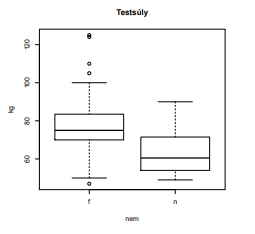
\includegraphics{boxplot}

(172) Irja rá az ábrára, hogy melyik tanult eloszláscsalád sűrűségfüggvényeit mutatják be és
egészítse ki a jelmagyarázatot is.

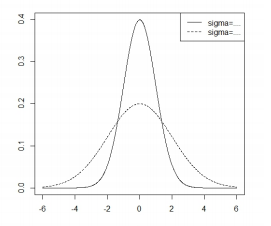
\includegraphics{fuggveny}

 Normális eloszlások (0 várható értékkel) a folytonos a standard, a szaggatott 2 szórású
(a sűrűségfüggvény képletét egybevetve az ábrával leolvasható)


(173) Miért volt érdemes az alábbi módon alkalmazni a hist függvényt? Rajzolja fel a függvény eredményét! 

\begin{verbatim}
hist(diak[,7],xlab="jegy",ylab="gyakoriság",main="Analízis
jegy",breaks=c(1:6)-1/2)
\end{verbatim}

Azért jó ez az intervallum-beosztás, mert így pontosan középre esnek a tényleges értékek
és nem keletkeznek "üres" oszlopok, amik a default beállításnál előfordulhatnak.

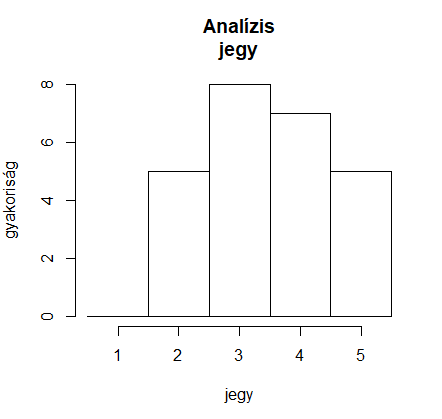
\includegraphics{histogram}

(174)  Mit vizsgáltunk? Mit kaptunk eredményül? Mi p.v jelentése?

\begin{verbatim}
p.v=rep(0,times=365);atlb=p.v;atlk=p.v
for (i in 1:365)
{jan1b<-homb[365*r+i,1];jan1k<-homk[365*r+i,1]
p.v[i]=t.test(jan1b,jan1k,paired=T,alternative="t")\$p.value
atlb[i]=mean(jan1b);atlk[i]=mean(jan1k)}
plot(p.v,type="l")
\end{verbatim}

p.v a p-értékek vektora az év napjaira. T-proba

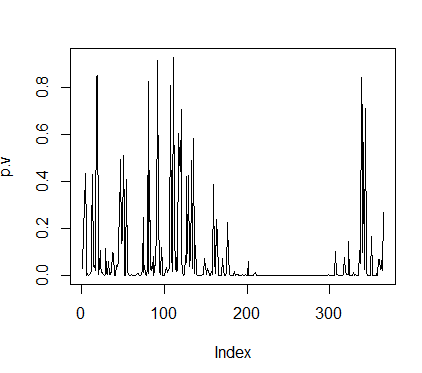
\includegraphics{pv}

(175) Milyen görbe van az ábrán? Milyen valószínúségszámítási tulajdonságai vannak?

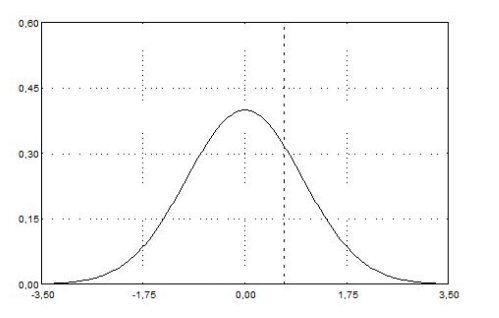
\includegraphics{gorbe}

ez standard normális eloszlás súrúségfüggvénye.


(176) Mit vizsgáltunk? Mit ad meg a p? Egészítse ki a táblázatot a hiányzó értékekkel!

\begin{verbatim}
n<-4;j<-6; q<-c(1:n)/n
h<-c(-Inf,qnorm(q)); mu<-mean(diak[,j])
sig=sd(diak[,j]) ; h<-h*sig+...
nu<-rep(0,times=n)
for (i in 1:n)
nu[i]<- sum((diak[,j]<h[i+1]) & (diak[,j]...h[i]))
np<-sum(nu)*rep(1/n,times=n)
c<-sum((nu-...)^2/np)
p<-1-pchisq(c,n-3)
\end{verbatim}

Lineáris modellt illesztettünk a
szeptemberi átlaghúmérsékletekre a nap sorszámának függvényében

A p a p-értéket jelöli.

Kiegészített változat:

\begin{verbatim}
n<-4;j<-6; q<-c(1:n)/n
h<-c(-Inf,qnorm(q)); mu<-mean(diak[,j])
sig=sd(diak[,j]) ; h<-h*sig+mu
nu<-rep(0,times=n)
for (i in 1:n)
nu[i]<- sum((diak[,j]<h[i+1]) & (diak[,j]>=h[i]))
np<-sum(nu)*rep(1/n,times=n)
c<-sum((nu-np)^2/np)
p<-1-pchisq(c,n-3)
\end{verbatim}

N jelentese a minták száma. $j$ a súly.


(177) Milyen statisztikai fogalmat illusztrál az ábra? Milyen tulajdonságai vannak?

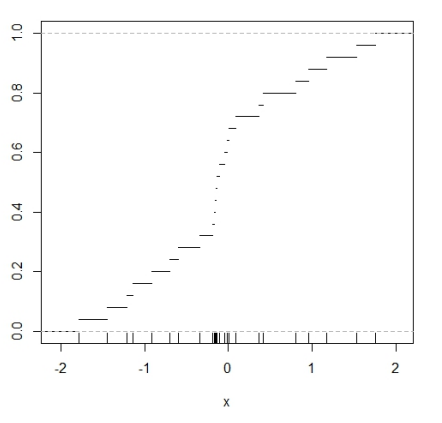
\includegraphics[scale=1.0]{gorbe2}

Ez standard normális eloszlású minta tapasztalati eloszlásfüggvénye.

\end{document}